\chapter{Introduction}
\label{chap:intro}

% TODO: updates to make:
% - 1.1 MIMO Channel overview
% 	- Add more discussion about MIMO CSI, capacity, precoding/beamforming, 
%	- Add details about 3GPP specificaions (possibly from latest preprint?)
% - Add more 

% Section \ref{sect:notation} introduces the notation used through this work.
This dissertation details work in improving the accuracy and efficiency of deep learning methods for MIMO channel state information estimation. This chapter provides the necessary background to understand the contributions of the dissertation. Section \ref{sect:mimo_model} provides an overview of the MIMO channel and the importance of CSI estimation in MIMO-based communications networks. Section \ref{sect:pilots} discusses the pilot reference signals used in CSI estimation. Section \ref{sect:channel_model} discusses MIMO channel models and introduces the primary channel model used in this work, the COST2100 model. Section \ref{sect:classic_estimation} discusses prior work in compressed sensing for CSI estimation.  
Boldface lowercase (uppercase) letters indicate vectors (matrices). Unless otherwise specified, the norm $\|\cdot\|$ indicates the Frobenius norm. Superscripts $^T$ ($^H$) indicate the transpose (Hermitian transpose).
% recent work in deep learning for CSI estimation in MIMO networks

\section{MIMO Channel Overview}
\label{sect:mimo_model}

\begin{figure}[!hbtp]
\centering
{
	\fontsize{6pt}{8pt}
	\def\svgwidth{0.8\columnwidth}
	\input{images/mimo-schematic.pdf_tex}
}
\caption{Example multi-antenna transmitter (BS, gNB) and single-antenna user equipment (UE) and relevant system values.}
\label{fig:mimo_schematic}
\end{figure}

In this work, we consider a MIMO channel with a multiple antennas ($N_B \gg 1$) at the transmitter (gNodeB or gNB) servicing a single user equipment (UE) with a single antenna. Under orthogonal frequency division multiplexing (OFDM) with $N_f$ subcarriers, the received symbols on the $m$-th subcarrier for the downlink and the uplink at the receiver are given as
\begin{align*}
	y_{d,m} &= \mathbf h_{d,m}^H\mathbf w_{t,m}x_{d,m} + n_{d,m}.
	% y_{u,m} &= \mathbf w_{r,m}^H\mathbf h_{u,m}x_{u,m} + \mathbf w_{r,m}^H\mathbf n_{u,m},
\end{align*}
where the individual system values are defined in Table~\ref{tab:mimo-params}, and a representative system model is viewable in Figure~\ref{fig:mimo_schematic}. The resulting downlink and uplink channel state information (CSI) matrices are given as
\begin{align*} 
	\bar{\mathbf H}_d &= \begin{bmatrix} \mathbf h_{d,1} & \dots & \mathbf h_{d,N_f}\end{bmatrix}^H \in \mathbb C^{N_f \times N_b}.
	% \bar{\mathbf H}_u &= \begin{bmatrix} \mathbf h_{u,1} & \dots & \mathbf h_{u,N_f}\end{bmatrix}^H \in \mathbb C^{N_f \times N_b}.
\end{align*}
\begin{table}[]
\renewcommand{\arraystretch}{1.25}
\centering
\caption{MIMO system variables considered in this work.}
\label{tab:mimo-params}
\begin{tabular}{c|c|l}
\toprule
\textbf{Symbol}   	  	  & \textbf{Dimension}            & \textbf{Description} \\ \midrule
$y_{d,m}$ 		  	  	  & $\mathbb{C}^{1}$ 			  & Received downlink symbol on $m$-th subcarrier  \\ \hline
$\mathbf h_{d,m}$ 	  	  & $\mathbb{C}^{N_b \times 1}$   & Downlink channel on $m$-th subcarrier  \\ \hline
$\bar{\mathbf H}_{d}$ 	  & $\mathbb{C}^{N_f \times N_b}$ & Downlink CSI (spatial-frequency domain)  \\ \hline
$\mathbf w_{t,m}$ 	  	  & $\mathbb{C}^{N_b \times 1}$   & Transmitter precoding vector for $m$-th subcarrier  \\ \hline
$x_{d,m}$ 		  	  	  & $\mathbb{C}^{1}$ 			  & Trasmitted symbol on $m$-th subcarrier  \\ \hline
$n_{d,m}$ 		  	  	  & $\mathbb{C}^{1}$ 			  & Downlink noise on $m$-th subcarrier  \\ \hline
$\tilde{\mathbf H}_{d}$   & $\mathbb{C}^{N_f \times N_b}$ & Downlink CSI (angular-delay domain)  \\ \hline
$\mathbf H_{d}$   		  & $\mathbb{C}^{R_d \times N_b}$ & Truncated downlink CSI (angular-delay domain)  \\ \hline
% $y_{u,m}$ 		  & $\mathbb{C}^{1}$ 			  & Received uplink symbol on $m$-th subcarrier  \\ \hline
% $\mathbf h_{u,m}$ & $\mathbb{C}^{N_b \times 1}$   & Uplink channel on $m$-th subcarrier  \\ \hline
% $\mathbf H_{u}$   & $\mathbb{C}^{N_f \times N_b}$ & Downlink impulse response on $m$-th subcarrier  \\ \hline
% $\mathbf w_{r,m}$ & $\mathbb{C}^{N_b \times 1}$   & Received precoding vector for $m$-th subcarrier  \\ \hline
% $x_{u,m}$ 		  & $\mathbb{C}^{1}$ 			  & Received symbol on $m$-th subcarrier  \\ \hline
% $\mathbf n_{u,m}$ & $\mathbb{C}^{1}$ 			  & Uplink noise on $m$-th subcarrier  \\ \hline
\end{tabular}
\end{table}
To achieve near-capacity transmission rates, the transmitter needs access to an appropriate estimate of $\bar{\mathbf H}_d$ \cite{ref:goldsmith2003capacity}. Such estimates enable the use of linear precoding techniques (e.g., conjugate beamforming or zero-forcing beamforming) to realize appreciable spectral and power efficiency gains \cite{ref:yang2013performance}. Downlink CSI estimation can be performed in time division duplex (TDD) by using uplink pilots due to channel reciprocity \cite{ref:Kaltenberger2010relative,ref:mi2017massive,ref:Gao2010utilization}. In contrast, frequency domain duplex (FDD) does not admit channel reciprocity due to frequency-selective channels, meaning CSI estimates must be acquired at the UE using pilot signals, and these estimates must be compressed then fed back to the BS.

\section{Practical Pilot-based Channel Estimation in 4G/5G Networks}
\label{sect:pilots}

% \section{Sparse Pilots in Practical Networks}
To estimate the downlink CSI in wireless networks, transmitters allocate pilot reference signals. To reserve spectral resources, pilots are restricted to a limited number of spatial-frequency positions, and the allocation of these pilots is defined in the 3GPP technical standards, TS 36.211 for 4G/LTE networks \cite{ref:3gpp.36.211} and TS 38.211 for 5G/NR networks \cite{ref:3GPPTS38.211V15.8.0}. In these two standards, the pilots are called CSI reference signals (CSI-RS) or demodulation reference signals (DM-RS), respectively. Figure~\ref{fig:lte-vs-5g} shows valid placements of CSI-RS/DM-RS in the time-frequency resource grid as defined by TS 36.211 and TS 38.211.

\begin{figure}[!hbtp]
    \centering
    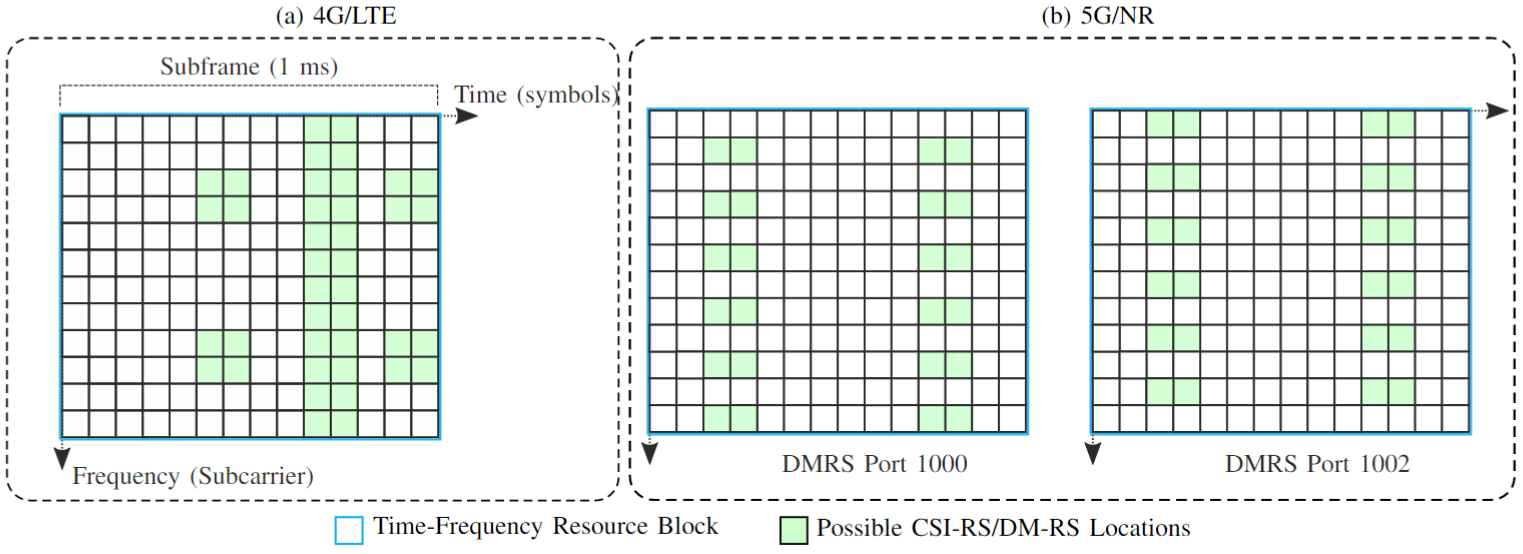
\includegraphics[width=\linewidth]{LTE_vs_5GNR_resource_grid.png}
    \caption{(a) LTE resource blocks with CSI-RS locations. (b) 5G NR resource blocks with DM-RS locations.}
    \label{fig:lte-vs-5g}
\end{figure}

For the UE to estimate the downlink channel state at the known pilot locations, the UE can use a straightforward least-squares estimator. Denote the pilot matrix $\mathbf{X}\in\mathbb{C}^{M_b \times \tau}$ where $\tau$ is a given number of timeslots that is less than the coherence interval of the channel. The received signal at the UE based on the transmitted pilots is,
\begin{align}
	\mathbf{y}_{\text{pilots}} &= \mathbf{h}_{\text{pilots}}\mathbf{X} + \mathbf{n},
\end{align}
where $\mathbf{h}_{\text{pilots}}\in\mathbb{C}^{1\times M_b}$ is the pilot matrix for a subset of the transmitter antennas such that $M_b < N_b$ and $\mathbf{n}\sim\mathcal{CN}(\mathbf{0},\sigma^2\mathbf{I})$ is additive complex Gaussian noise. Pilot estimation based on $\mathbf{y}_{\text{pilots}}$ and $\mathbf{X}$ is straightforward using the least-squares solution,
\begin{align}
	\hat{\mathbf{h}}_{\text{pilots}} &= \mathbf{y}_{\text{pilots}}\mathbf{X}^H(\mathbf{X}\mathbf{X}^H)^{-1}. \label{eq:pilots-least-squares}
\end{align}
While many works using deep learning for CSI estimation do not address pilot estimation explicitly (i.e., they assume perfect CSI at the UE), a few such works have incorporated pilot estimation into the CSI feedback problem. These works typically apply deep learning to either A) improve upon the least-squares estimator of (\ref{eq:pilots-least-squares}) or B) design the pilot matrix, $\mathbf{X}$. In \cite{ref:mashhadi2021pruning}, the authors propose a fully-connected network (FCN) which performs pilot allocation and coarse CSI estimation followed by a CNN-based attention layer for refining the estimate, and they proposed architecture, and the authors demonstrate the efficacy of the proposed network compared to the MMSE estimator as well as other neural estimators. In \cite{ref:sohrabi2021distributed}, the authors propose to incorporate a trainable pilot design as a portion of an end-to-end model that directly maps pilots at the UE into feedback bits and then feeds those received bits at the BS into a precoding matrix, thereby avoiding explicit CSI estimation.

In this dissertation (namely, in Chapter~\ref{chap:p2d}), we propose an estimator of the truncated delay domain CSI (see Section~\ref{sect:sparse-csi} of Chapter~\ref{chap:sph_norm}) based on the sparse frequency domain pilots (i.e., $\hat{\mathbf{h}}_{\text{pilots}}$ of equation (\ref{eq:pilots-least-squares}) above).

\section{Geometric Stochastic Channel Models (GSCMs)}
\label{sect:channel_model}

Ideally, the datasets used for the CSI estimation task would be derived from measurement campaigns (e.g., see \cite{ref:shepard2016argoschannel,ref:du2021interuserangle,ref:li20222finegrained}). However, the financial and labor costs of acquiring these datasets can be prohibitive in certain situations. In such situations, researchers use geometric stochastic channel models (GSCMs), models which are so called since they consider the \textbf{geometry} of scatterers in the wireless environment and the \textbf{stochastic} nature of the channel. Simulations based on GSCMs are advantageous to researchers for a a few reasons:
\begin{enumerate}
	\item Simulations permit the generation a large quantities of data in a (relatively) short period of time.
	\item Simulations enable the adjustment of parameters of the communications system (e.g., carrier frequency, UE mobility, subcarrier spacing).
\end{enumerate}

GSCMs consider the problem of modeling the wireless channels at two different scales. At a small-scale, the focus is on the modeling of ``scatterers,'' objects in the environment which reflect the electromagnetic waves transmitted during. Examples of scatterers in an outdoor environment are buildings, balconies, cars, and trees, while examples of scatters in an indoor environment are walls, furniture, and people. Due to the presence of many scatterers, electromagnetic waves transmitted from a BS arrive at UEs along multiple paths at different delays, and accordingly, the scatterers are often referred to as \textbf{multipath components (MPCs)}. From the UE's perspective, the MPCs are often grouped together in specific delay regions, and each such grouping of MPCs is referred to as a \textbf{cluster}. In GSCMs, modeling is done at a cluster-level, capturing the diverse effects of many MPCs that are present in typical real-world wireless channels. Modeled clusters are typically parameterized by three values: delay, direction of departure (DoD), and direction of arrival (DoA).  

While the modeling of MPCs and clusters is vital, also vital is ensuring that the results of the GSCM-based simulations are statistically consistent with the measured channel data. This consistency is ensured by selecting \textbf{large-scale parameters (LSPs)}, examples of which are the delay spread and the angular spread. In designing GSCMs, the goal is to balance the fidelity of cluster behavior (based on delay, DoD, DoA) and of LSPs when compared to measured channel data. In practice, researchers implement GSCMs based on two different modeling approaches: system-level modeling or cluster-level modeling.

In system-level modeling, the interaction(s) between the BS and the UE(s) is first defined by choosing LSPs. This selection of LSPs is done by sampling from probability distributions. Based on the LSPs, the clusters and MPCs for each BS/UE interaction is defined.

While some well-known channel models, such as the 3GPP Spatial Channel Model (SCM) \cite{ref:3gpp.25.996} and  WINNER II \cite{ref:kyosti2007winner}, adopt the system-level approach, this modeling approach has some salient limitations. First, system-level models do not lend themselves well to high-mobility scenarios, as the LSPs are likely to change as the position of UEs change substantially. Second, system-level models make the addition of new LSPs (e.g., inter-link correlation) to a given interaction.

In contrast with system-level models, cluster-level models begin with cluster/MPC definition then move on to LSPs. First, a large number of clusters are defined by sampling from a chosen probability distribution. Then, the location(s) of UE(s) is (are) defined, and the scattering of each cluster is calculated based on the ``visibility'' of UEs with respect to the clusters. Finally, the LSPs are synthesized by sampling from a given probability distribution.

The cluster-level approach addresses both of the issues associated with system-level approaches. Simulating time-varying channels with high mobility is straightforward since it involves recalculating UE visibility and LSPs, and layering new LSPs into the model is simple since it is the last step of the simulation.

For all CSI tests, we mainly rely on a cluster-level GSCM, the COST2100 channel model,  \cite{ref:liu2012cost2100}. We use two datasets with a single base station (gNB) and a single user equipment (UE) in the following scenarios:
\begin{enumerate}
	\item \textbf{Indoor} channels using a 5.3GHz downlink at
	0.001 m/s UE velocity, served by a
	gNB at center of a $20$m$\times 20$m coverage area.
	\item \textbf{Outdoor} channels using a 300MHz downlink at 0.9 m/s UE velocity served by a gNB at center 
	of a $400$m$\times 400$m coverage area.
\end{enumerate}
In both scenarios, we use the parameters listed in Table~\ref{tab:cost-params}.
\begin{table}[]
\centering
\caption{Parameters used for COST2100 simulations for both Indoor and Outdoor datasets.}
\label{tab:cost-params}
\begin{tabular}{c|c|l}
\toprule
\textbf{Symbol} & \textbf{Value} & \textbf{Description} \\ \midrule
$N_b$ 			& 32			 & Number of antennas at gNB  \\ \hline
$N_f$ 			& 1024			 & Number of subcarriers for OFDM link  \\ \hline
$R_d$ 			& 32			 & Number of delay elements kept after truncation  \\ \hline
$N$ 			& $10^6$		 & Total number of samples per dataset  \\ \hline
$T$ 			& 10		 	 & Number of timeslots  \\ \hline
$\delta$		& 40 ms			 & Feedback delay interval between consecutive CSI timeslots  \\ \bottomrule
\end{tabular}
\end{table}

\section{Classical CSI Estimation}
\label{sect:classic_estimation}

Works in compressive feedback for CSI estimation in MIMO networks can be placed in three broad categories. The first category includes works which use direct quantization of continuous CSI elements to discrete levels. The quantized CSI are encoded and fed back to the transmitter \cite{ref:makki2012hybrid,ref:shirani2009channel}. The second category includes works which use compressed sensing, a technique which applies a random measurement matrix at the transmitter and the receiver \cite{ref:rao2014distributed, ref:eltayeb2014compressive}. Compressed sensing assumes matrices to be encoded and fed back meet certain sparsity requirements, and compressed sensing algorithms require iterative solvers \cite{ref:do2008sparsity} for decoding, resulting in undesired latency.

The last category of work in compressive CSI feedback uses deep learning (DL), neural networks with numerous layers which are trained on large datasets using backpropagation. We will provide the background knowledge needed for deep learning in Chapter 2, Section~\ref{sect:dl_overview}.

\section{Objective and Contributions}

Successful efforts in DL for CSI estimation have typically utilized convolutional neural networks (CNNs) in an autoencoder structure \cite{ref:csinet}. Variations on the CNN-based autoencoder have investigated different network architectures \cite{ref:Lu2020CRNet}, variational training frameworks \cite{ref:Hussien2020PRVNet}, and denoising modules \cite{ref:Sun2020AnciNet}. These architectural changes are largely inspired by successful application of DL in image compression \cite{ref:szegedy2017inception,ref:balle2017end,ref:xie2012image}.

While they can continue to push the state-of-the-art in CSI reconstruction accuracy, architectural optimizations may ultimately follow the same trends of fields such as language modeling, where state-of-the-art performance requires prohibitively massive compute (e.g., \cite{ref:brown2020language}). In comparison to the massive compute used in such NLP tasks, the compute available in CSI estimation is much more limited, as these CSI estimation networks are (partially) deployed on UEs. 
% In this proposal, we take a different approach seek to improving compressive channel feedback by focusing on domain knowledge and physical insight.
% While the powerful functional approximation of deep CNNs has enabled state-of-the-art CSI reconstruction accuracy, they run the risk falling into the same trap as the image.

Rather than focus solely on architectural optimizations or large compute, this dissertation details our attempts to use domain knowledge to enhance the performance and the efficiency of neural networks for CSI estimation. Chapter~\ref{chap:sph_norm} details provides more background information on DL for CSI estimation as well as our work in power-based normalization, which leverages CSI sparsity to improve performance. Chapter ~\ref{chap:markovnet} describes our work in differential encoding, which exploits temporal coherence of CSI to improve estimation performance while providing a less complex network than recurrent neural network-based CSI estimation networks. Chapter~\ref{chap:p2d} describes our work in pilot-based delay domain CSI estimation, where we draw an explicit link between frequency-domain CSI estimation as defined in 3GPP specifications and the delay domain CSI used in many DL-based CSI estimation works. For a visual summary of these contributions and the respective areas of domain knowledge we leverage, see the Venn diagram in Figure~\ref{fig:contrib})

\begin{figure}[htb] \centering 
	{
	  \fontsize{6pt}{6pt}
	  \def\svgwidth{1.0\columnwidth}
	  \input{images/cnns-venn-diagram-contrib-final.pdf_tex}
	}
	\caption{Venn diagram highlighting different aspects of domain knowledge in CNN-based CSI compressive feedback, relevant convolutional networks, and our contributions.}
	\label{fig:contrib}
\end{figure}